Rather than be built as a monolithic block, CowHub has a number of small, modular components that serve different purposes and form a complete system; CowHub is a system of loosely-connected micro-services. Each and every component is deployable separately, having been built and tested independently and corresponds to a source repository on GitHub. Each component can be dependent on other services in the system, but these are mocked during the testing stage and implemented fully in production. For an overview of all important components, see Figure \ref{fig:structure}.

\begin{sidewaysfigure}
  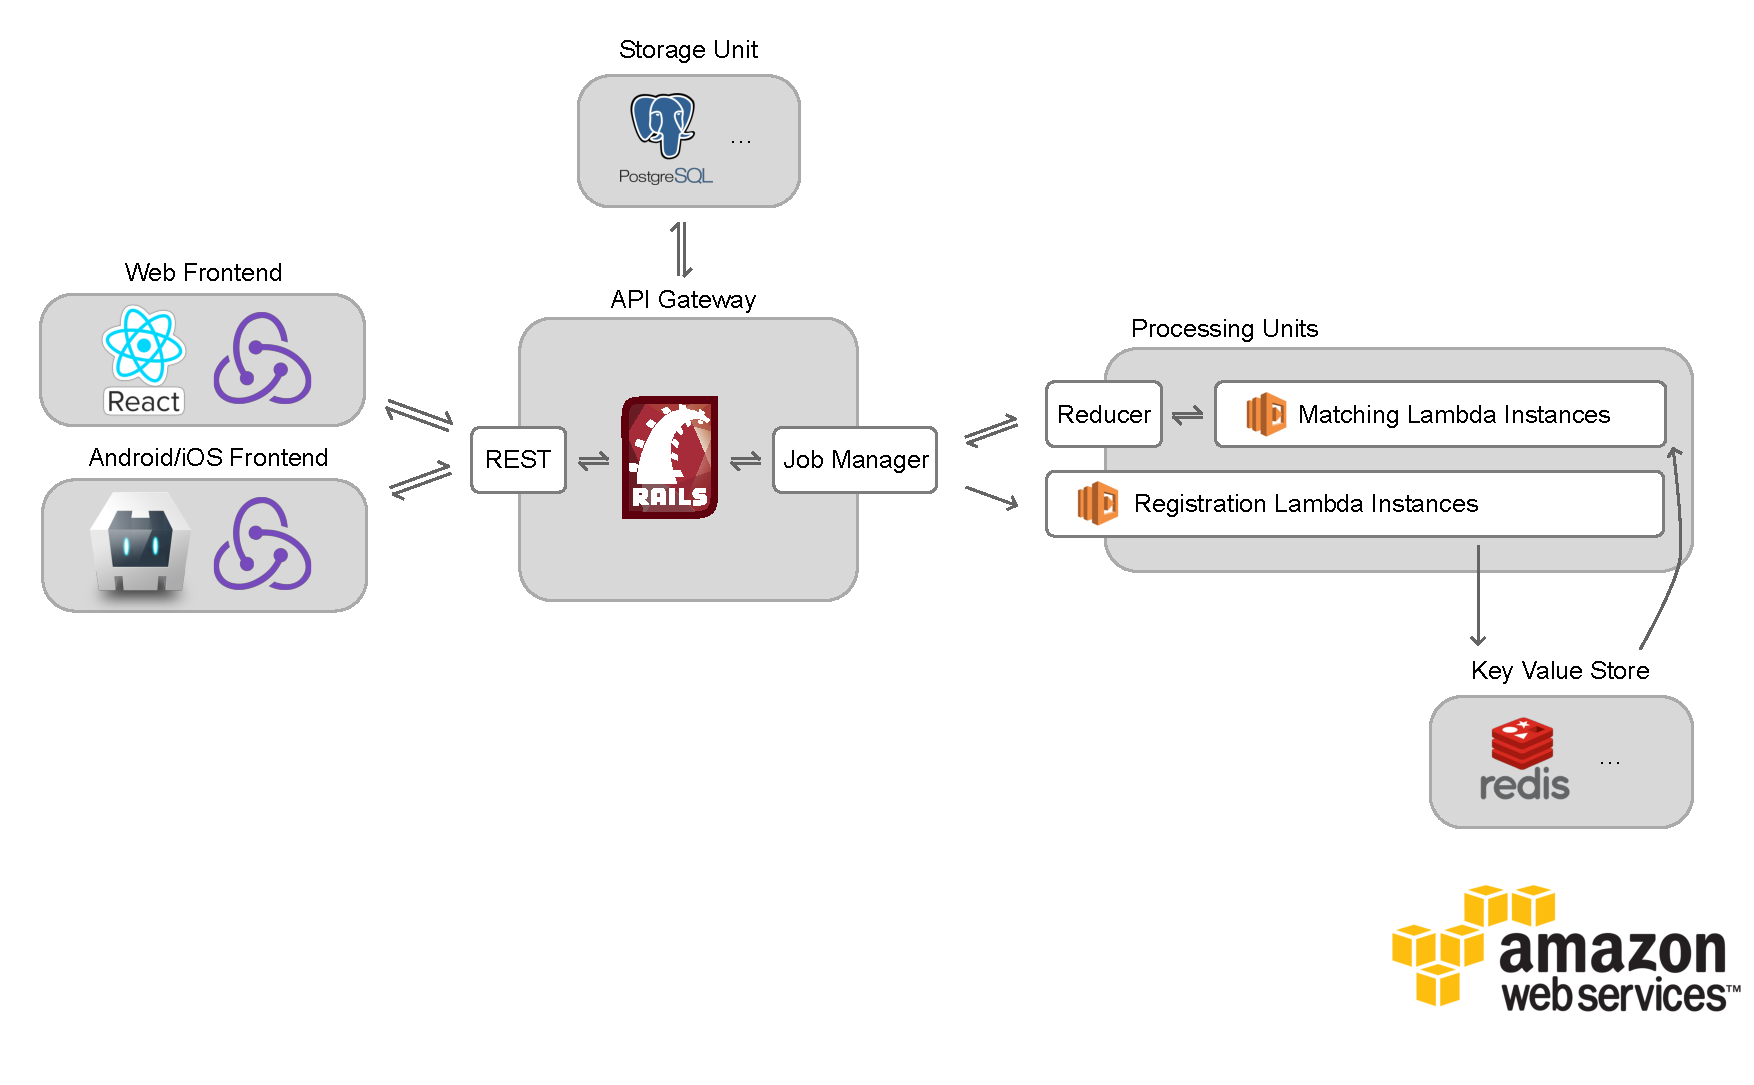
\includegraphics[width=\textwidth]{sketch/structure.pdf}
  \caption{The structure of CowHub}
  \label{fig:structure}
\end{sidewaysfigure}

CowHub uses Amazon Web Services (AWS) for a scalable, robust and stable cloud solution. For this project, the used services include IAM, CloudFront, Route 53, VPC, EC2, S3, RDS, Lambda, ElastiCache and API Gateway\footnote{This will later be referred to as Amazon API Gateway for disambiguation.}. The use of each service will be explained further in the following report.

The report proceeds with respect to the components of the project.

\subsection{Persistent Data Storage}
Persistent storage for the application is built on top of Amazon Relational Database Service (RDS) and Amazon Simple Storage Service (S3). PostgreSQL has been chosen to be the engine for the database service. The database unit aims to provide a simple, scalable and cloud-based database interface for our other services to use.

RDS has been chosen because it is an easy solution to a resizable and scalable database, and provides features such as duplication. By employing RDS we could focus more on the application that we are building and pay little to no attention to the time-consuming database administrative tasks.

S3 is used to hold all file and blob data. It has been chosen because of its persistent, simple, durable infrastructure and more importantly, its integration with other Amazon and CowHub services.

The database is to store the following:

\begin{enumerate}
	\item The information about farm and farmers. 
	\item The information about registered cattle, including the herd number, (optionally) the name, the owner, the birthdate, and most importantly the sample image(s) of its muzzle for identification uses.
	\item The login details of registered farmers. Farmers will need to log in to be able to input and review the cattle data.
	\item The match results. Every match job will be assigned a job ID and the result will be stored into the database. These match results will be useful in the future as statistics.
	\item Other data for the system to run smoothly (including session tokens etc.). 
	% TODO: more stuff about databases
\end{enumerate}

The database unit is only accessible through the API Gateway\footnote{Images are encoded in Base64 format before transfer (as a string).}.

\subsection{API Gateway}
The API Gateway (API) can be thought of as the centre of the system, and is written in Ruby on Rails (RoR). RoR has enabled us to prototype and implement the component in an elegant and efficient manner; its seamless integration with Rspec has also allowed us to test the component more efficiently\footnote{Nearly all sub-components have automated tests and are integrated with the continuous integration and delivery system.}.

The API has two most important subcomponents:

\begin{enumerate}
	\item A REST API for communication with the front-ends.
	\item A Job Manager for communication with the headless computational unit.
\end{enumerate}

The REST API mainly handles the following:

\begin{enumerate}
	\item Account management. A user (farmer) needs to be able to manage his/her personal data, change passwords and etc.
	\item Cattle management. A user (farmer) needs to be able to create/edit/delete information about a cattle and upload/update/delete images for a cattle. 
	\item Session management. The API handles sessions through tokens in a unified manner for all front-ends that require user login as REST API is stateless.
	% TODO: more stuff about our API
\end{enumerate}

We have a standardised URL schema for the API that allows us to develop the component more efficiently.

The Job manager is the more interesting part. There are two different types of jobs:

\begin{enumerate}
	\item Cattle registration job. For this type of job, an anonymous job is created (the result is not saved into the database). This is required because we do not match image with image; instead we used an edge descriptor to mathematically describe the muzzle of a cattle. The registration job is to deal with the descriptor generation so that we do not have to calculate the descriptor every time it is required.
	\item Cattle matching job. A job ID is required for this type of job as 1) we need to be able to track the status of the ongoing job and 2) we need to save the match result for statistical purposes. The process, roughly, includes (in the following order):
	\begin{enumerate}
		\item Generate the descriptor for the image to be matched.
		\item Divide the database of images into chunks with size $N$\footnote{A predefined value. For the proof of concept we have chosen 25.}, label each chunk with an ID $\text{id}_i$.
		\item For each chunk with ID $\text{id}_i$, forward the ID, the job ID and the image descriptor to the headless computational unit and wait for a best match within the chunk to be handed back. The headless computational unit will run asynchronously for all calls.
		\item Aggregate the result for a best match. Write the best match into the database and return it to the caller.
	\end{enumerate}
\end{enumerate}

Based on our statistics, step (a) normally takes a half to one second, and every pairwise match in step (c) takes about 30 to 80 milliseconds\footnote{This is due to the resizing and normalisation done prior to the match.}. That is, ignoring the network and IO delays, a match will take about $T = N * t_m / 1000 + t_d / 1000$ seconds to complete, where $t_m \in [30, 80]$ and $t_d \in [500, 1000]$. In this reasoning our computation time can be thought of as upper bounded by $Nc$, where $c \in \mathbb{Q}$, which is totally size-agnostic, because it is based on the assumption that we would always have $\lceil M / N \rceil$ computational units at our disposal. This rational implies that, in theory, the computation time does not generally grow with respect to the number of images in our database\footnote{In practice it does - because we cannot ignore the time consumed for IO actions.}.

\subsection{Key Value Store}
A cluster of Redis servers is employed through Amazon ElastiCache service. 

For performance reasons it has been decided that we use a key value store for concurrent and lively access for the descriptor of an image. This store is to be accessed very frequently and as only a small piece of data is being extracted at once it seemed inappropriate to be using a database. Another reason that a key value store is used, as opposed to accessing the descriptor directly from the database unit is data separation - the only place that this data is being accessed is the headless computational unit and nothing more. Also, as suggested before, the database unit is only accessible through the API, and any access directly from other components would break the promise; alternatively, to access the descriptors through the API would introduce significant (and unnecessary) burden to the API itself and result in great performance problems.

\subsection{Headless Computational Unit}
The processing is built on top of AWS Lambda services. The headless computational unit supports two different kinds of jobs: registration and matching, as suggested before. A call to the headless computational unit will cause a Lambda calculation unit (Lambda) to be spawned. Lambda processes are running concurrently, and they are not necessarily on the same machine\footnote{It can be thought of as Actors - universal primitives for concurrent computation. Similar constructs implementation include \textit{Akka} for Scala.}.

The two different kinds of the Lambda processes include:

\begin{enumerate}
	\item Registration Lambda. This is a one way communication. The caller (the API) calls the headless computational unit, causing a Registration Lambda to be spawned. This Lambda process will run to the end (the generation of the descriptor of an image) and then store it into the Key Value store.
	\item Matching Lambda. The caller will need to call the headless computational unit with the job detail, and the Matching Lambda will run the match for $N$ images as discussed before. This process is running concurrently. Upon finishing the process, the Lambda will forward the best match within a batch of $N$ images back to the caller as notification.
\end{enumerate}

The process of matching is similar to that of Map Reduce, and so is the implementation. The only difference, through the use of AWS Lambda, is that we do not provision or administer the servers ourselves - the computational units are spawned ad hoc and only whenever needed.


\subsection{Mobile and Web Front-ends}
Our mobile application supports Android and iOS platforms. There is no plan on supporting Windows Phone in the foreseeable future.

To assist the development process in a rather short period of time, we have decided to use a cross-platform solution to build our app on. More specifically, we have employed Apache Cordova \cite{cordova} framework as the foundation block of our app, and most of the application level programming is done in JavaScript. This implies that our apps have the so-called ``hybrid'' structure where

\begin{itemize}
	\item the interface prototyping is done in a unified manner, in JavaScript and styling in CSS - meaning that it will produce the same layout across different platforms because the interface is shown through a WebView\footnote{An important assumption made here is that the WebView will behave uniformly for the subset of layout techniques that we have used. Thanks to the use of WebKit rendering engine on both platforms and the standardised protocols and guidelines for the Web this assumption can be, to a degree, thought as true.};
	\item most of the higher level logic is written in JavaScript, giving the same behaviour cross-platform, meaning that we can start the development without any prior platform-specific knowledge;
	\item agile development of the application is allowed as there is little to none compilation required for the application to be built;
	\item most of the Node.js libraries are made available for use: React.js and Redux, for example;
\end{itemize}

The use of the the ``hybrid'' structure also yields certain disadvantages compared to developing the application natively. For example, the performance will, to some extent, suffer from the extensive use of WebView, and so will the battery life; access to low-level and platform dependent features are limited, and requires more fiddling\footnote{Normally through the native interface of the framework.} for it to work. But clearly for the amount of time given, and the state of the framework those disadvantages are out-weighted by the advantages listed above.

The Web front-end is coded using React.js and Redux, and there is no server side rendering required. For our Web front-end to work there only needs to be a server serving static files, thus making our Web front-end highly performant and scalable.

The front-ends are all stateless, meaning that they will run independently. Another important implication is that users can develop their own front-end easily, should they feel that the provided front-ends are not for their taste.

\subsection{Implementation Difficulties And Comments}

% TODO: finish the implementation difficulties section

\subsubsection{Headless Computational Unit}

One serious issue is here is performance, especially in the thinning process\footnote{Zhang-Suen thinning algorithm.} as the computational task is quite substantial. In this special case, it is required to inline C++ code as opposed to having pure Python code for the thinning iteration\footnote{The inline version runs within 600ms with IO whereas the pure Python version just times out after 10 seconds.}. The recommended approach is to use \texttt{weave} from \texttt{scipy} to inline the small piece of code. However this has proven to be not so easy: Amazon Lambda has a (code) package size limit of 250MB, and \texttt{scipy} itself is over 200MB - this implies that there is no way that we can use \texttt{scipy}.

It has come to us that since we only need to use \texttt{weave} and according to the official documentation, it can be installed as an independent library. Weird enough, it turns out that \texttt{weave} uses \texttt{scipy} internally - meaning that we will not be able to use \texttt{weave} at all.

The only way that's left then is to manually compile the C++ code into an object file for Python to use. Fortunately this is not too difficult: all we need to do is to run the code with \texttt{weave.inline} on a compatible machine and grab the \texttt{weave}-generated C++ file from the cache and for every platform we compile it into an object file and leave it inside the \texttt{lib} directory. This works because \texttt{weave} generates the boilerplate for seamless Python integration. After this step we would be able to replace the code with a call to the generated function in the generated module and remove the requirements for \texttt{weave} and \texttt{scipy}.

\subsubsection{Maintaining Security}

% TODO: Maintaining security comments

\subsubsection{Infrastructure Financial Constraints}

% TODO: Infrastructure financial constraints

\subsubsection{Keeping The API Gateway Performant} 

% TODO: Keeping the API Gateway Performant
